\documentclass{article}
\usepackage{graphicx}
\usepackage[margin=1in]{geometry}
\usepackage{amsmath}
\usepackage{xcolor}
\usepackage{titlesec}
\usepackage[scaled=0.96]{helvet} % Sets up Helvetica font
\definecolor{mauve}{rgb}{0.58,0,0.82}

\titleformat{\section}[hang]{\color{mauve}\normalfont\sffamily\Large}{\thesection}{1em}{}
\titleformat{\subsection}[hang]{\color{mauve}\normalfont\sffamily\large}{\thesubsection}{1em}{}


\title{Homework 1}
\author{Anshul Sawant}
\date{Due date: Feb 1 at 11:59 PM}

\begin{document}
\maketitle

\section*{Question 1.2 (10 points)}
\subsection*{A}
Let $\theta(t) = \pi \frac{t - a}{b - a}$. Then:
\[
lr(t)=
\begin{cases}
    lr_{max} \frac{t}{a},& \text{if } t < a\\ 
    lr_{min} + (\cos{\theta(t)} + 1)\frac{lr_{max} - lr_{min}}{2},& \text{if } a < t \leq b
\end{cases}
\]
\subsection*{B}
Cosine annealing can lead to more stable training because of:
\begin{enumerate}
\item Warm up, which is known to stabilize transformer training.
\item Higher initial and lower final training rate ensures fast learning initially and more stable learning afterwards.
\end{enumerate}
\section*{Question 1.3 (9 points)}
\subsection*{A}
Validation loss for GPT-tiny is 7.048.
\subsection*{B}
The loss had not saturated at 2000 steps.
\subsection*{C}
See Figure \ref{fig:loss}.
\begin{figure}
\centering
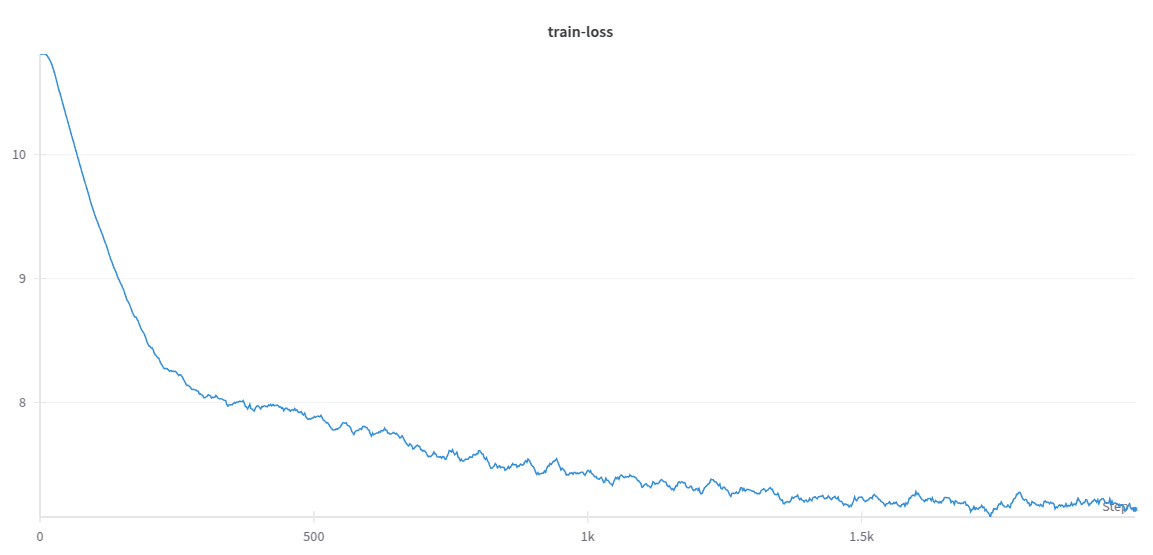
\includegraphics[totalheight=6cm]{training_loss.png}
\caption{GPT-tiny training loss}
\label{fig:loss}
\end{figure}
\section*{Question 1.4}
\subsection*{A}
Experiment procedure was random hyperparameter search with:
\begin{verbatim}
n_positions = seq_len
grad_accumulation_steps = 1
num_warmup_steps = num_training_steps/10
max_lr = 10 * min_lr
batch_size in {32, 64, 128, 256, 512}
n_positions in {32, 64, 128, 256, 512}
n_head in {2, 4, 8}
n_embd in {64, 128, 256, 512}
n_layer in {2, 4, 6, 8}
n_training_steps determined by FLOP limit
min_lr in {1e-3, 5e-4, 1e-4, 5e-5, 1e-5}
\end{verbatim}
 Number of training steps were calculated based on allowed flops. We rejected model size less than 50 MB and more than 98 MB. The smaller models were rejected because it is known that larger models perform better. Models that lead to GPU OOM were naturally, rejected.
\subsection*{B}
Following trends are observerd:
\begin{enumerate}
\item More heads are preferred (4 or 8 over 2).
\item More layers are preferred (4 or 6 over 2).
\item Large model dimension is preferred (256 over all others).
\item Large batch size is preferred (128 or 256 over 32 or 64).
\item Since the model is still pretty small, large learning rates are okay.
\item While we would like batch size and model size to be as large as possible, these are counter balanced by the limits on model size and GPU memory.
\end{enumerate}
At the top end of the spectrum, validation perplexity ranged between 225 and 275.
\subsection*{C}
First I tried the best model from the above. However, the model saturated too soon and I could get a validation loss of 4.4 which lead to perplexity about the cutoff.
\begin{verbatim}
output_dir: outputs/full_training 
input_file: tokens.npz
tokenizer_encoding: gpt2         
model_config:
  n_embd: 256                   
  n_head: 8                    
  n_positions: 32             
  n_layer: 4                      
device: auto                 
batch_size: 256             
seq_len: 32                
num_warmup_steps: 12590   
num_training_steps: 125900
grad_accumulation_steps: 1
min_lr: 5e-4             
max_lr: 5e-3            
\end{verbatim}
Thereafter, based on what I know about models and the patterns I saw from the random search, I decided to train a pretty much as large a model as possible with a pretty big batch size (256 x 4 gradient accumulation steps). This lead to required performance. The model config is as follows:
\begin{verbatim}
output_dir: outputs/full_large
input_file: tokens.npz
tokenizer_encoding: gpt2
model_config:
  n_embd: 256
  n_head: 8
  n_positions: 64
  n_layer: 8
device: auto
batch_size: 256
seq_len: 64
num_warmup_steps: 1259
num_training_steps: 12590
grad_accumulation_steps: 4
min_lr: 0.0005
max_lr: 0.005
\end{verbatim}
I got a validation set perplexity of 41.2.
\end{document}
